\documentclass[a4paper,12pt]{article}
\usepackage[margin=1in,left=1in,includefoot]{geometry}
%\usepackage{amsmath}
\usepackage[tbtags]{amsmath}%%%%%https://tex.stackexchange.com/questions/368353/using-equation-split-how-can-i-ensure-that-only-the-last-equation-is-numbered%%%%
%%%%%%%%%%%%%%%%%%%%%%%%%
\usepackage[utf8]{inputenc}
\usepackage{fontspec}
 %\usepackage{enumitem}
 %%%%%%%%%%%%%%%%%%%%
 \usepackage{amsmath}
 \usepackage{amsfonts}
 \usepackage{amssymb}
\usepackage{mathtools}
\usepackage{amsthm}
\everymath{\displaystyle}
%%%%%%%%%%%%%%%%%%%%%%%%%%%%%%%%%%%%
\usepackage{ragged2e}%%%%%%%%%%%%%%for \justify
%%%%%%%%%%%%%%%%%%%%%%%%%%%%
\usepackage[dvipsnames]{xcolor}
\usepackage{xcolor}
\usepackage{booktabs,tabularx}
\usepackage{multirow}
\usepackage{tikz}
\usepackage{graphicx} % Required for including images
\usepackage[font=small,labelfont=bf]{caption} % Required for specifying captions to tables and figures
%%%%%%%%%%%%%%%%%%%%%%%%%%%%%%%%
\usepackage[colorlinks=true]{hyperref}%
 %%%%%%%%%%%%%%%%%%%%%%%%%%%%%%%%%%%%%
\usepackage[ethiop,main=english]{babel}
\newfontface{\geezfont}{FreeSerif}
\newenvironment{geez}{\geezfont}{}
\lccode`፡=`፡  \catcode`፡=11
\lccode`።=`። \catcode`።=11
\babelprovide[import,
  onchar = fonts ids,
  typography/intraspace = 0 .1 0,
  typography/linebreaking = s, 
  characters/ranges = 1200..139F 2D80..2DDF AB00..AB2F,
  ]{amharic}
\babelfont[amharic]{rm}{FreeSerif}
%%%%%%%%%%%%%%%%%%%%%%%%%%%%%%%%%%%%%%%%%%%%%%%%
%%%%%%%%%%%%%%%%%%%%%%%%%%%%%%%%%%%%%%%%%%%%%%%%%%%%
%\newtheoremstyle{mystyle}%                % Name
%  {}%                                     % Space above
%  {}%                                     % Space below
%  {\itshape}%                             % Body font
%  {}%                                     % Indent amount
%  {\bfseries}%                            % Theorem head font
%  {.}%                                    % Punctuation after theorem head
%  { }%                                    % Space after theorem head, ' ', or \newline
%  {}%                                     % Theorem head spec (can be left empty, meaning `normal')
% 
%%%%%%%%%%%%%%%%%%%%%%%%%%%%%%%%%%%%%%%%%%%%%%%%%%%%%%%%%%%%%%%%%%%%%
%`\usepackage{newcent} % Default font is the New Century Schoolbook PostScript font 
%\usepackage{helvet} % Uncomment this (while commenting the above line) to use the Helvetica font
%%%%%%%%%%%%%%%%%%%%%%%%%%%%%%%%%%%
%\usepackage[many]{tcolorbox}
%%%%%%%%%%%%%%%%%%%%%%%%%%%%%%%%%%%%%%%%%%%%%%%%%%%%%%%%%%%%%%%%%%%%%
%\theoremstyle{mystyle}
%\newtheorem{theorem}{Theorem}
%\newtheorem{proposition}{Proposition}
%\newtheorem{lemma}{Lemma}
%\newtheorem{corollary}{Corollary}
%\newtheorem{example}{Example}
%\newtheorem{solution}{Solution}
%\newtheorem{conclusion}{Conclusion}
%\newtheorem{definition}{Definition}
%\newtheorem{remark}{Remark}
%%%%%%%%%%%%%%%%%%%%%%%%%%%%%%%
%\tcolorboxenvironment{definition}{
%    enhanced jigsaw, pad at break*=1mm, breakable,
%    left=4mm, right=4mm, top=1mm, bottom=1mm,
%    colback=red, boxrule=0pt, frame hidden,
%    borderline west={0.5mm}{0mm}{red}, arc=.5mm
%}
%%%%%%%%%%%%%%%%%%%%%%%%%%%%%%%%%%%%%%%%%%%%%%%%%
%\numberwithin{equation}{section}
%\numberwithin{theorem}{section}
%\numberwithin{proposition}{section}
%\numberwithin{example}{section}
%\numberwithin{remark}{section}
%\numberwithin{lemma}{section}
%\numberwithin{corollary}{section}
%\numberwithin{definition}{section}
%%%%%%%%%%%%%%%%%%%%%%%%%%%%%%%%%%%%%%%%%%%%%%%%%%
%%%%%%%%%%%%%%%%%%%%%%%%%%
\usepackage[shortlabels]{enumitem}
%\usepackage{soul}%%for highlighting texts and equations begin inside $$..\hl{some text here}
\newcommand{\mathcolorbox}[2]{\colorbox{#1}{$\displaystyle #2$}}%%to highlight math equations which is inside \begin{equation}...\end{equation}
%%%%%%%%%%%%%%%%%%%%%%%%%%%%%
%\usepackage[tbtags]{amsmath}%%%%%https://tex.stackexchange.com/questions/368353/using-equation-split-how-can-i-ensure-that-only-the-last-equation-is-numbered%%%%
%%%%%%%%%%%%%%%%%%%%%%%%%
%%%%%%%%%%%%%%%%%%%%%%%%%%%%%%%%%%%%%%%%%%%%%%%%%%%%%%%%%%%%%%%%%%%%
\usepackage[backend=bibtex,maxnames=1000,minnames=10,maxalphanames=1000,
minalphanames=10,style=numeric,sorting=anyt,firstinits=true]{biblatex}
\DeclareNameAlias{default}{last-first}
\addbibresource{volume-1-book-25.1.1.bib}
\renewbibmacro{in:}{}
%%%%%%%%%%%%%%%%%%%%%%%%%%%%%%%%%%%%%%%%%%%%%%%%%%%%%%%%%%%%%%%%%%%%%%
%%%%%%%%%%%%%%%%%%%%%%%%%%%%%%%%%%%%%%%%%%%%%%%%%%%%%%%%%%%%%%%%%%%%%
%opening
%\title{
%{\bf \large A research proposal}\\[3mm]\large by\\[2mm]Dagnachew Jenber\\[3mm]On\\[2mm]{\bf \large A strongly convergent algorithm to the solution of split common fixed point problem for strict quasi-G-pseudocontractive mappings and Bregman strict quasi-$D_f$-pseudocontractive mappings in Banach spaces using generalized f-projection operator and Bregman generalized f-projection operator respectively }}
%\author{}
%\date{}
\usepackage{geometry}
\usepackage{graphicx}
\title{{\color{blue}\begin{geez}\Huge 0 ወይም 1\end{geez}}\\
{\color{blue}\par\noindent\rule{\textwidth}{1.5pt}}\\[3mm]
{\large \begin{geez}\Huge ዜሮ ወይም አንድ ትሬዲንግ አክሲዮን ማህበር\end{geez}}
{\color{blue}\par\noindent\rule{\textwidth}{1.5pt}}}
\author{\bf \begin{geez}ዳኛቸው ጀንበር ነጋሽ\\[3mm]የደራሲው የግል ድህረ-ገፅ፡ \url{https://dagnachewjenber.github.io/Dagnachew-Jenber/} \end{geez}}
%Supervisors:\\[3mm]
%{\bf Prof. Habtu Zegeye Hailu}\\
%Department of Mathematics \& Statistical Sciences,\\
%Faculty of Sciences, BIUST, Botswana\\[3mm]
%{\bf Mollalgn Haile Takele (PhD, Assistance Professor)}\\
%Department of Mathematics, Bahir Dar University, Ethiopia\\[3mm]
%{\bf Abebe Regassa Tufa (PhD, Assistance Professor)}\\
%Department of Mathematics, University of Botswana, Botswana}
\date{~~~~}
% Definition of \maketitle
\makeatletter         
\def\@maketitle{
\raggedright
%%%
%%%
%%%
\centering
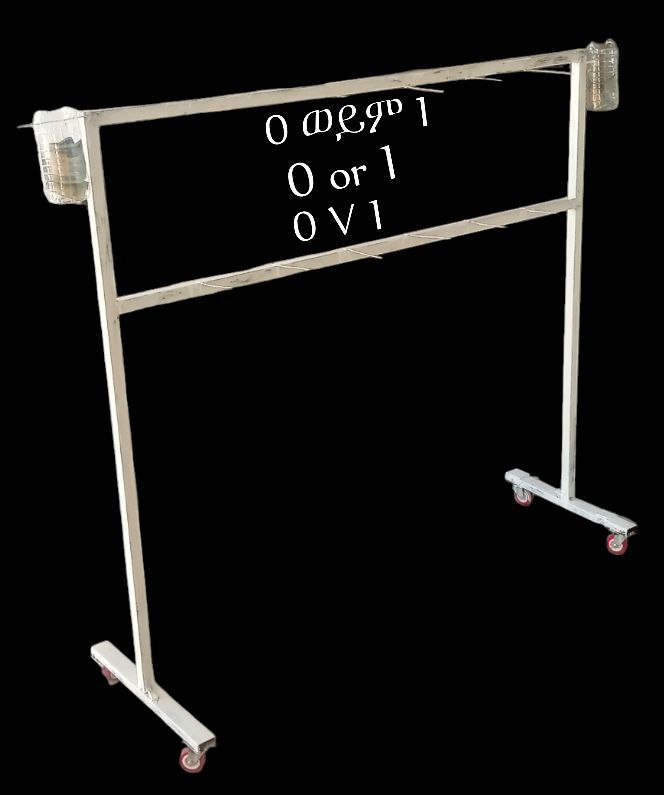
\includegraphics[width = 40mm]{0_or_1.jpg}\\[1.5ex]
\begin{center}
{\large \bfseries \sffamily \@title }\\[1.5ex] 
{  \@author}\\[1.5ex] 
\@date\\[8ex]
%\includegraphics[width = 40mm]{image.png}
\end{center}}
\makeatother
%%%%%%%%%%%%%%%%%%%%%%%%%%%%%%%%%%%%%%%%%%%%%%%
%%%%%%%%%%%%%%%%%%%%%%%%%%%%%%%%%%%%%%%%%%%%%%%%%%
%\makeatletter
%\renewcommand*\l@section{\@dottedtocline{1}{1.5em}{2.3em}}
%\makeatother

\makeatletter
\renewcommand\tableofcontents{%
  \null\hfill\textbf{\Large\contentsname}\hfill\null\par
  \@mkboth{\MakeUppercase\contentsname}{\MakeUppercase\contentsname}%
  \@starttoc{toc}%
}
\makeatother
%%%%%%%%%%%%%%%%%%%%%%%%%%%%%%%%%%%%%%%%%%%%%%%%%%%
%%%%%%%%%%%%%%%%%%%%%%%%%%%%%%%%%%%%%%%%%%%%%%%%%%%%%
\usepackage{hyperref}% http://ctan.org/pkg/hyperref
\usepackage{footmisc}
\hypersetup{%
  colorlinks = true,
  linkcolor  = blue,
  citecolor=red,
  urlcolor=blue
}
%%%%%%%%%%%%%%%%%%%%%%%%%%%%%%%%%%%%

%%%%%%%%%%%%%%%%%%%%%%%%%%%%%%%%%%%%%%
%%%%%%%%%%%%%%%%%%%%%%%%%%%%%%%%%%%%%%%%
\usepackage[absolute,overlay]{textpos}  
%\newcommand{\ethnum}[1]{#1}%%%chatGpt: how can I adjust the numbering of each section and subsection in \ethnum in Latex? Thank you!!!
\renewcommand{\thesection}{\ethnum{\arabic{section}}}
\renewcommand{\thesubsection}{\thesection.\ethnum{\arabic{subsection}}}
\renewcommand{\thesubsubsection}{\thesubsection.\ethnum{\arabic{subsubsection}}}
%%%%%%%%%%%%%%%%%
\usepackage{titlesec}%%chatGpt: would you tell me how to increase the font size of section and subsection part in latex
\titleformat{\section}{\fontsize{20}{24}\bfseries}{\thesection}{1em}{}
\titleformat{\subsection}{\fontsize{18}{22}\bfseries}{\thesubsection}{1em}{}
%%%%%%%%%%%%
\renewcommand{\contentsname}{ማውጫ}%%replaces ``content'' in the pdf output of \tableofcontents by ``ማውጫ''.
%\hypersetup{bookmarksopen=true,pdfstartview={FitH},pdfbookmark[1]{ማውጫ}{toc}}%update PDF bookmarks
\begin{document}
\large
%\fontspec{Abyssinica SIL}
%\fontfamily{Sans Serif}
%\fontfamily{kpfonts}
\maketitle
\thispagestyle{empty}
\vfill
\begin{minipage}[t]
{0.5\textwidth}
\raggedright
\textcopyright\ \begin{geez}ዳኛቸው ጀንበር ነጋሽ፣ 2017 ዓ.ም\end{geez}
\end{minipage}
\begin{minipage}[t]
{0.5\textwidth}
\raggedleft
\date{\begin{geez}2017 ዓ.ም\end{geez}}
\end{minipage}
%%%%%%%%%%%%%%%%%%%%%%%%%%%%%%%%%%%%%%%%%%%%%%%%%%%%%%%%%
\renewcommand{\thefootnote}{}%remove numbering for the footnote
\footnotetext{\scriptsize \textcopyright\ The Author(s) 2025. Open Access This article is licensed under a Creative Commons Attribution-NonCommercial-NoDerivatives
4.0 International License, which permits any non-commercial use, sharing, distribution and reproduction in any medium or format, as long as you give appropriate credit to the original author(s) and the source, provide a link to the Creative Commons licence, and indicate if you modified the licensed material. You do not have permission under this licence to share adapted material derived
from this article or parts of it. The images or other third party material in this article are included in the article’s Creative Commons licence, unless indicated otherwise in a credit line to the material. If material is not included in the article’s Creative Commons licence and your intended use is not permitted by statutory regulation or exceeds the permitted use, you will need to obtain
permission directly from the copyright holder. To view a copy of this licence, visit \url{https://creativecommons.org/licenses/by-nc-nd/4.0/}.}
\renewcommand{\thefootnote}{\arabic{footnote}}%%restore default numbering for future footnotes
\clearpage
\pagenumbering{roman} % Use lowercase Roman numerals
\tableofcontents
\clearpage
%\endgroup   % end of TeX group
%%%%%%%%%%%%%%%%%%%%%%%%%%%%%%%%%%%%%%%%%%%%%%%%%%%%%%%%%%%%%%%%%%
%%%%%%%%%%%%%%%%%%%%%%%%%%%%%%%%%%%%%%%%%%%%%%%%%%%%%%%%%%%%%%%%%
%\hypersetup{
%  colorlinks= true,
%  citecolor=red,
%  linkcolor=blue,
%  urlcolor=blue}  
%\hypersetup{
%  citebordercolor=red,
%  filebordercolor=red,
%  linkbordercolor=blue}
%\begin{center}
%\begin{minipage}{.9\linewidth}
%\begin{center}
%A research Project
%\end{center}
%\begin{center}
%On
%\end{center}\bf
%An iterative algorithms for split common fixed point problem in Banach spaces
%\end{minipage}
%\end{center}
%\begin{center}
%By
%\end{center}
%\begin{center}
%Dagnachew Jenber Negash\\Bahir Dar University, Department of mathematics\\Addis Ababa Science and Technology University, Department of Mathematics\\
%Email: dagnachew.jenber$@$aastu.edu.et
%\end{center}
\pagenumbering{arabic} % Reset page numbering to Arabic numerals
\section{\begin{geez}መግቢያ\end{geez}}
\label{s:1}
\subsection{\begin{geez}0 ወይም 1 ባጭሩ ሲገለፅ\end{geez}}
0 ወይም 1 በሚከተሉት ነገሮች ይገለፃል።
\begin{itemize}
\item ጨዋታ፣
\item ትምህርት፣
%\item ቁማር፣
\item ሽልማት፣
\item ንግድ።
\end{itemize}
\subsection{\begin{geez}ተልእኮ\end{geez}}
የ 0 ወይም 1 ጨዋታ ተልእኮ እንደሚከተለው ነው። 
\begin{itemize}
\item ለማህበረሰቡ የተለያዩ ትምህርቶችን በአዛምድ መልክ እየተዝናኑ እንዲያውቁ ማድረግ። ለምሳሌ የአንድን እንግሊዘኛ ቃል በአማርኛና በሌላ ተመሳሳይ ቃላቶች በጨዋታ እየተዝናኑ እንዲያውቁ ማድረግ። ስለዚህ በዚህ መልኩ ተመራማሪ እና አንባቢ ማህበረሰብን ማፍራት ይቻላል። ምክኒያቱም ከጉዋደኞቹ ጋር ተወዳድሮ ለማሸነፍ ወይም ጨዋታውን ለማሸነፍ እንዲሁም ያሸነፈበትን ገንዘብ ለመውሰድ ሲል ብዙ ያነባል። ከዚህ በተጨማሪ በጨዋታ መልክ የተማሩት ነገር የመረሳት ዝንባሌው ትንሽ ነው።
\item ማህበረሰባዊ ተግባቦትን መጨመር። ይህን ጨዋታ ለብቻ መጫወት ቢቻልም ከሰው ጋር ሆነው ሲጫወቱት ግን ይበልጥ ያምራል። ከዚህ በተጨማሪም በተጫዋቾች መካከል ውይይትን ይፈጥራል።
\end{itemize}
\subsection{\begin{geez}ራእይ\end{geez}}
የ 0 ወይም 1 ጨዋታ ራእይ እንደሚከተለው ነው።
\begin{itemize}
\item አንባቢ ማህበረሰብን ማፍራትና አዳዲስ እውቀትን ማስጨበጥ ነው።
\item በሆነ ጉዳይ ላይ ማህበረሰባዊ ውይይትን ማሳደግ።
\end{itemize}
\section{\begin{geez}ለመፍታት የታሰበው ችግር\end{geez}}
\subsection{\begin{geez}የችግሩ መግለጫ\end{geez}}
የችግሩ መግለጫ (statement of the problem) እንደሚከተለው ባጭሩ እናስቀምጠዋለን።
\begin{itemize}
\item የአንባቢያን ማህበረሰብ እየቀነሰ መምጣት። በብዙ ምክኒያት ሰወች ቁጭ ብለው ማንበብ የተውበት ጊዜ ነው። ከብዙወቹ ምክኒያቶች ውስጥ ጠቃሚ ያልሆነ ሶሻል ሚዲያ ላይና በልባሌ ቦታወች ጊዜን ማጥፋት የተለመደ ሆኗል።
\end{itemize}
\subsection{\begin{geez}የችግሩ መፍትሔ\end{geez}}
\begin{enumerate}
\item ማንበብን ወይም ጥናትን መዝናኛና ገንዘብ ማግኛ እንዲሁም ደግሞ ሽልማት የሚያስገኝ ማድረግ። ከማጥኛ ወይም አዲስ እውቀትን ከማግኛ  ዘዴወች ውስጥ አንደኛው ነገሮችን በተመሳሳያቸው በማዛመድ ማወቅ ነው። ለምሳሌ የአንድ እንግሊዘኛ ቃል ብዙ ተመሳሳይ ቃላቶች አሉት። እነሱን በማዛመድ ለመሸምደድ መሞከር ጥሩ ከሚባሉት ዘዴ ውስጥ አንዱ ነው። ግን ደግሞ ይሄን ልምምዶሽ አይረሴ ለማድረግ በጨዋታ መልክ ሆኖ በቡድን እየተዝናኑና እየተወያዩ ሲሆን ተመራጭ ያደርገዋል። 
 ለምሳሌ ካርድ በማዘጋጀት የእንግሊዘኛ ቃላቶችን ማጥናት በሚል ዙሪያ የተጠኑ ሳይንሳዊ ጥናቶች አሉ (ለምሳሌ፣ እነዚህን ይመልከቱ፣ \cite{aslan2011teaching,azabdaftari2012comparing,bryson2012using,kosim2013improving,
 nikoopour2014vocabulary,
nugroho2012improving,
saputri2017improving,senzaki2017reinventing,sitompul2013teaching,
wahyuni2014flashcards}) 
\item ነገሮችን በአይነት አይነታቸው እያዛማዱ ማወቅ ያመራምራል፣ ጠያቂ ያደርጋል፣ ከጓደኛ ጋር ያከራክራል፣ ማመሳከሪያ መፅሃፍ ፍለጋ እስከመሄድ ድረስ ያደርሳል። እናም በዚህ መልክ ሲሆን ያን ነገር ለመርሳት ብዙ ጊዜ ይጨርሳል። 
\item ማዛመድን ደግሞ ከጉዋደኛ ጋር ሆነው እየተዝናኑ በጨዋታ መልክ ካደረጉትና እውቀትንና ማወቅን ለማበረታት ደግሞ ለአሸናፊው ጉርሻ በመስጠት ከሆነ ጨዋታውም ተወዳጅ ይሆናል ማለት ነው።
\item ከላይ ከ1-3 የተጠቀሱትን መፍትሔወች ለማከናወን የተለያዩ አይነት ጨዋታወችን ማዘጋጀት። 
\end{enumerate}
\section{\begin{geez}የገበያው ምርመራ\end{geez}}
\subsection{\begin{geez}ደንበኞች\end{geez}}
\begin{itemize}
\item ይህ ገበያ በማንኛውም እድሜ ክልል ያለን ያሳትፋል። በጨዋታ መልክ የተዘጋጀ ስለሆነና በአይነቱ ደግሞ አዲስና አስተማሪ የሆነ ስለሆነ ብዙ ደንበኞች ይኖሩታል ተብሎ ይታመናል። 
\end{itemize}
\subsection{\begin{geez}ተወዳዳሪ ሓይላት\end{geez}}
\begin{itemize}
\item በኢኮኖሚ የዳበሩ ግለሰቦች ወይም ድርጅቶች ይሄን የገበያ ሞዴል የመወዳደር አቅም አላቸው። ምክኒያቱም የገንዘብ ችግር ስለሌላቸው ባንድ ፀሃይ ግባት ገበያውን ማጥለቅለቅ ይችላሉ።  
\end{itemize}
\subsection{\begin{geez}መጠንና የመስፋት አቅም\end{geez}}
\begin{itemize}
\item ብዙ የአክሲዮን ባለድርሻ አካላትን የሚያሳትፍ ስለሚሆን በመጠን ሰፊ ነው። ይህ አክሲዮን በብዛት መምህራንን የሚያሳትፍ ስለሚሆን በመጠኑ እየሰፍ የሚሄድ ይሆናል ተብሎ ይታመናል።
\item ይህ ገበያ በውስጡ ብዙ አይነት ለወደፊቱ እየተፈለሰፉና እየዳበሩ የሚሄዱ የጨዋታ ሞዴሎችን ስለሚይዝ በመላው ኢትዮጵያ ይስፋፋል ተብሎ ይታመናል።
\end{itemize}
\section{\begin{geez}0 ወይም 1 ጨዋታ ሞዴል\end{geez}}
የሚከተለው ምስል 1 የ 0 ወይም 1 ጨዋታ መጫወቻ ቴብል ሲሆን ከዚህ በተጨማሪም የዜሮ ወይም አንድ ትሬዲንግ አክሲዮን ማህበር መለያ አርማም ነው። ምስል 2 ደግሞ የ 0 ወይም 1 መጨወቻ ቴብል ምስል 1 ልኬቷን በሴንቲ ሜትር ያሳያል።
\begin{center}
\begin{figure}[h!]
\centering
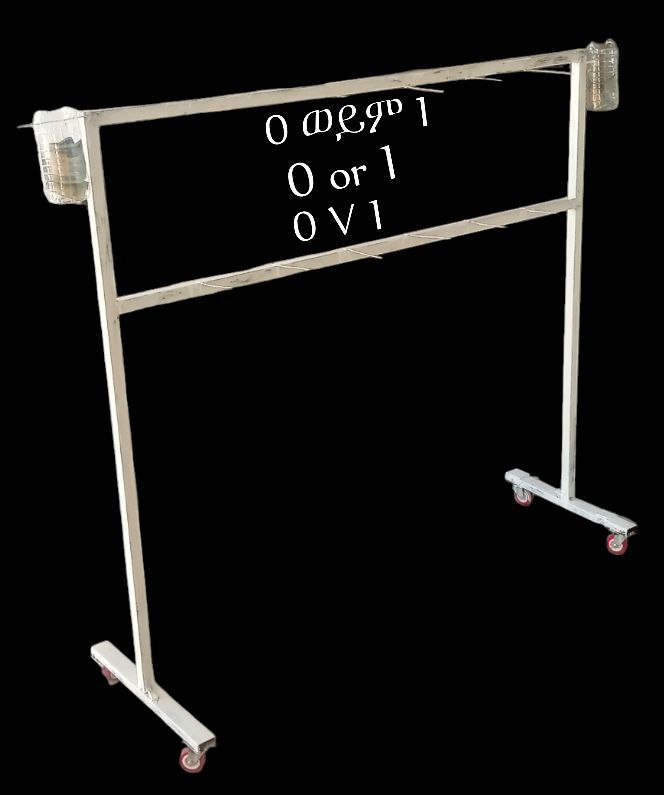
\includegraphics[scale=0.3]{0_or_1}
\caption{ምስል 1: የ 0 ወይም 1 መለያ አርማ (logo)}
\end{figure}
\end{center}
\newpage
\begin{center}
\begin{figure}[h!]
\centering
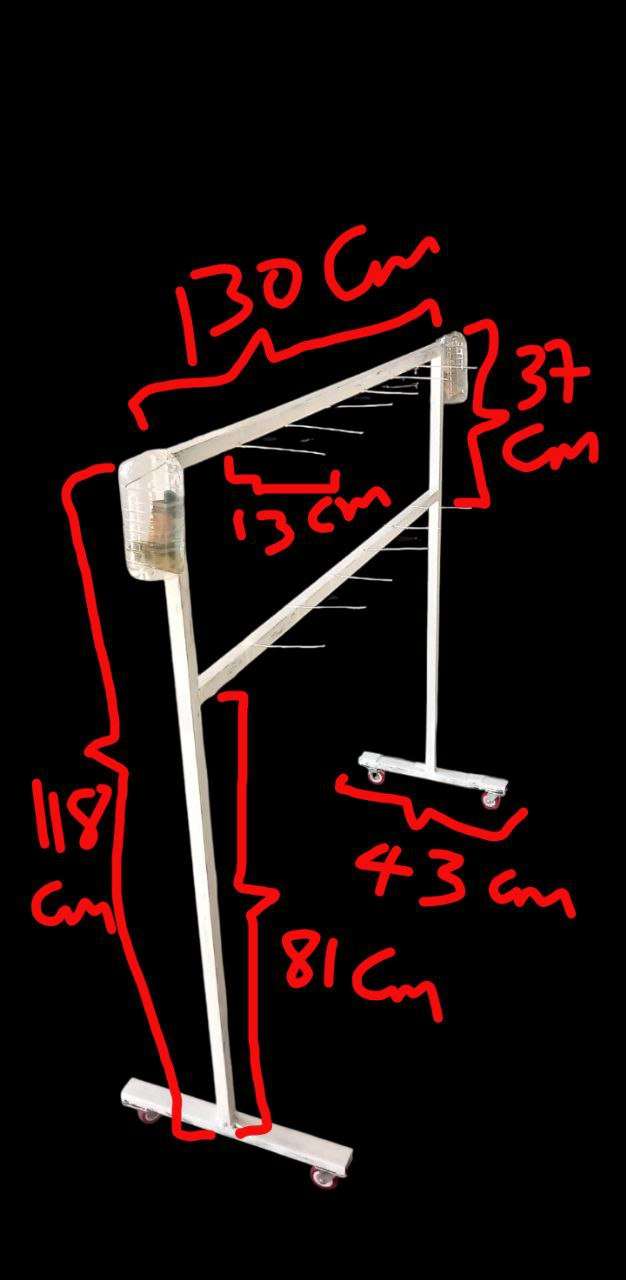
\includegraphics[scale=0.3]{0or1}
\caption{ምስል 2: የ 0 ወይም 1 መጫወቻ ምስል 1 ልኬት}
\end{figure}
\end{center}
\subsection{\begin{geez}መስሪያ እቃወች\end{geez}}
\begin{enumerate}
\item ብረት ወይም እንጨት፣
\item የወረቀት ካርዶች።
ስለዚህ 0 ወይም 1 የሚባለው የጨዋታ ሞዴል በብረት (ወይም በእንጨት) እንዲሁም ደግሞ ከወረቀት ካርዶች በቀላል ወጭ የሚሰራ የጨዋታ አይነት ነው።
\end{enumerate}
{\color{red}ማስታወሻ}፡ የ 0 ወይም 1 ጨዋታ ማጫወቻ ቴብል  2 መርፌ፣ 3 መርፌ፣ 4 መርፌ ፣ ወዘተ ሊኖረው ይችላል። ከላይና ከታች ያሉት መርፌወች ብዛት አንድ አይነት ነው። ባለ 2 መርፌ ስንል ከላይና ከታች ያለውን ቆጥረን ሳይሆን የላይኛውን ብቻ ቆጥረን ነው። ለምሳሌ ከላይ ያለው ስእል ባለ 6 መርፌ ይባላል። ታችኛው ድርቡ አይቆጠርም።
\subsection{\begin{geez}የካርድ አዘገጃጀት\end{geez}}
\begin{itemize}
\item \justify ካርዶችን በ Latex እናዘጋጃቸዋለን። ቀላል የሆነ Latex ነው የምንጠቀመው። የ Latex template ስላለ ለማንኛውም የካርድ አዘጋጅ ሰራተኛ ይሰጠዋል። የካርዱ መጠን የ A4 ወረቀት አንድ አራተኛ ነው።
\end{itemize}
\begin{itemize}
\item \justify ካርዶቹን በደረጃ እንከፋፍላቸዋለን። ማለትም ደረጃ 0.1፣ ደረጃ 0.2፣ ወዘተ እያልን እንከፍላቸዋለን። ለምሳሌ ጠቅላላ እውቀት (general knowledge) ካርዶችን general knowledge 0.1፣  general knowledge 0.2፣ general knowledge 0.3፣ ወዘተ እያልን እንከፋፍለዋለን። 
\end{itemize}
\begin{itemize}
\item \justify General knowledge 0.1፣ ወዘተ እያሉ የሚቀጥሉት ካርዶች ማንኛውንም እውቀት የሚያጠቅልሉና ሰፊ ናቸው። General Knowledge 1.1፣ ወዘተ እያሉ የሚቀጥሉት ግን ከአንደኛ ክፍል የትምህርት አይነቶች የተውጣጡ  ጠቅላላ እውቀት  ናቸው። General Knowledge 2.1፣ ወዘተ እያሉ የሚቀጥሉት ደግሞ ከሁለተኛ ክፍል የትምህርት አይነቶች የተውጣጡ  ጠቅላላ እውቀት  ናቸው።  ሌላው  ምሳሌ ደግሞ የ 1ኛ ክፍል English ትምህርት ካርዶችን  English 1.1, English 1.2, English 1.3, ወዘተ እያልን እንከፋፍለዋለን። ለሌሎችም የትምህርት አይነትና የክፍል ደረጃ እስከ ዩኒቨርስቲ ድረስ በዚህ መልኩ ካርዶች ይዘጋጃሉ ማለት ነው።
\end{itemize}
\begin{itemize}
\item \justify የካርዶች ብዛት ከአጫዋች ካርዶች በስተቀር የ 8 ብዜት እንዲሆኑ ለማድረግ የሚከተለውን እናደርጋለን። አጫዋች ካርዶች የሚባሉት ከላይኛው መርፌወች የሚቀመጡት ናቸው። የመርፌወች ብዛትና የአጫዋች ካርዶች ብዛት እኩል ነው። ለምሳሌ ባለ 6 መርፌ 0 ወይም 1 ጨዋታ ቴብል ቢኖረን የአጫዋች ካርዶች ብዛትም 6 ነው ማለት ነው።  ስለዚህ "n" ን የካርድ ብዛት ይሁን ብንል "p" ን የመርፌው ብዛት ይሁን ብንል "k" ን ደግሞ የ 8 ማብዣ ይሁን ብንል "n" ን ለማግኘት የሚከተለውን ቀመር እንጠቀማለን ምክኒያቱም "p" እና "k" የተሰጡ ናቸው የሚፈለገው "n" ብቻ ይሆናል ማለት ነው። 
$$n=8k+p።$$
ለምሳሌ የመርፌው ብዛት፣ p=6 ቢሆን፤ የ 8 ማብዣ ደግሞ፣ k=2 ይሁን ብንል። ስለዚህ $n=8k+p=8(2)+6=22$ ይሆናል ማለት ነው።
\end{itemize}
\begin{itemize}
\item {\color{red}ማስታወሻ}፤ የካርዶች ብዛት የ 8 ብዜት እንዲሆን የተፈለገበት ምክኒያት አጨዋወት በሚለው ክፍል ውስጥ ገለፃ ይደረግበታል። 
\end{itemize}
\subsection{\begin{geez}አጨዋወት\end{geez}}
0 ወይም 1 ጨዋታን ለመጫወት ደረጃ 0.1፣ ደረጃ 0.2፣ ወዘተ ተብለው የተዘጋጁ ካርዶችና ዋናው ቴብል ያስፈልጋል። ከደረጃ 0.1 ወደ ደረጃ 0.2 ስንሄድ የካርዱ ብዛት እየጨመረ ይሄዳል። ጨዋታውን ለብቻ ወይም በቡድን መጫወት ይቻላል።
\begin{enumerate}
\item[(ሀ)]{\color{red}ለብቻ መጫወት}-ይሄን ጨዋታ አንድ ሰው ብቻውን ሊጫወተው ይችላል ግን አሰልች ነው። ምክኒያቱም ተወዳዳሪ ከሌለህ ደስ አይልም ልክ ብቻን ፑል እንደመጫወት ነው የሚሆነው ስሜቱ።
\end{enumerate}
\begin{enumerate}
\item[(ለ)] {\color{red}ለቡድን መጫወት}-አንዱ ካርድ ዋጋ ይተመንለትና በካርዱ ልክ አጫዋቹ በተጫወቾቹ ይከፈለዋል።\\
{\color{blue}$\bullet$} ለምሳሌ 18 ካርድ ብዛት ካለና የአንዱ ካርድ ዋጋ 1 ብር ከሆነና ሰወቹ ስድስት ሆነው መጫወት ከፈለጉ እያንዳንዳቸው 3 ብር በማዋጣት ይከፍሉና ጨዋታውን መጫወት ይችላሉ።
\end{enumerate}
\begin{enumerate}
\item[(ሐ)] {\color{red}እርስ በርስ መሸላለም}- ተጫዋቾች ጨዋታውን እርስ በርስ በመሸላለም ማድረግ ከፈለጉ ተነጋግረው በፈለጉት ብር መጠን መጫወት ይችላሉ። ለምሳሌ ባጠቃላይ 18 ካርድ ካለና ስድስት ተጫዋቾች ካሉና እያንዳንዳቸው መቶ ብር አዋተው ቢጫወቱ ሁሉንም የመለሰ ጨዋታውን ያሸንፋል። ለምሳሌ ከስድስቱ ውስጥ አንድ ሰው ካሸነፈ፤ አሸናፊው 6*100=600 ብር ይበላል። ሁለት ሰወች ካሸነፉ 600 ብር ለሁለት ይካፈሉትና 300 ብር እያንዳንዳቸው ይደርሳቸዋል። 3 ሰወች ካሸነፉ እያንዳንዳቸው 600/3=200 ብር ይደርሳቸዋል። 4 ሰወች ካሸነፉ 600/4=150 ብር ይደርሳቸዋል። 5 ሰወች ካሸነፉ እያንዳንዳቸው 600/5=120 ብር ይደርሳቸዋል። ስድስቱም ሰወች ካሸነፉ እያንዳንዳቸው 600/6=100 ብር ይደርሳቸዋል። ማንም ካላሸነፈ ጨዋታውን እንደገና ይጫወታሉ። እንደገና መጫወት ያልፈለገ የስያዘውን ብር መልሶ ይዞ መውጣት ይችላል። አንድ ተጫዋች ጨዋታውን ለማሸነፍ ሞዴሉ ላይ እንዳየነው ሁሉንም የአዛምድ መልስ መመለስ አለበት።
\end{enumerate}
{\color{blue}$\bullet$} ጨዋታው በሚከናወንበት ጊዜ ሁሌም የተንቀሳቃሽ ምስል ቀረፃ አለ። ማለትም ሁሉም የ 0 ወይም 1 ጨዋታ በአጫዋቹ ይቀረፃል። የጨዋታው ቀረፃ በ youtube ይለቀቃል። ስለዚህ ማንኛውም ፍላጎት ያለው የተጫወተውን ጨዋታ youtube ላይ ገብቶ ማየት ይችላል፣ ከተጫወቱ በኋላ ማጭበርበር አይችሉም፤ እንደ ማስታወሻም ይሆናል፣ ወላጆችም ልጆቻቸውን youtube ላይ በማየት መገምገም ይችላሉ፣ ልጆችም ካደጉ በኋላ እንደማስታወሻ ሊጠቀሙበት ይችላሉ፣ ወዘተ ብዙ ጥቅም አለው።\\
{\color{blue}$\bullet$} {\color{red}ማስታወሻ፤} አንድ ተጫዋች አንድን ካርድ ለማስቀመጥ የ 0 ወይም 1 ጨዋታ ቴብሉ በያዘው የመርፌ (pin) ብዛት ሲባዛ በሁለት ሴኮንድ ይሰጠዋል። ለምሳሌ ከላይ እንዳለው ስእል ቴብል ከሆነ እንደምታዩት የመርፌ ብዛቱ 6 ነው፣ ስለዚህ አንድን ካርድ ለማስቀመጥ 12 ሴኮንድ ይሰጠዋል ማለት ነው።
\begin{enumerate}
\item[(መ)] {\color{red}ውርርድ}-ተመልካቾች የውርርድ ጨዋታ መጫወት ይችላሉ። ለምሳሌ 6 ተጫዋቾች ካሉና ደረጃ 0.1 መጫወት ፈለጉ እንበል። ደረጃ 0.1 ደግሞ 18 ካርዶች አሉት እንበልና ይሄን ጨዋታ ተጫውተው ለመጨረስ ደግሞ እያንዳንዳቸው ተጫዋቾች 3 ካርድ ይደርሳቸዋል። ከመጀመሪያው ወደ ኋላኛው ተጭዋቾች 1፣2፣3፣4፣5፣6 ተብለው ይሰየማሉ። ለምሳሌ ቁጥር-1 ተጫዋች የመጀመሪያውን ካርድ ስቦ አዛምዱን ሊሰራው ይችላል። አዛምዱን ሲሰራው 1 ይባላል። ሁለተኛውን ካርድ ስቦ ደግሞ አዛምዱን ላይሰራው ይችላል፣ አዛምዱን ካልሰራው 0 ይባላል። ይህ ተጫዋች አሁንም ሶስተኛውን ካርድ ስቦ አዛምዱን ሊሰራው ይችላል፣ በዚህ ጊዜ 1 ይባላል። ስለዚህ በቅደም ተከተል ቁጥር-1 ተጫዋች 101 ሆኖ ጌሙን ተሸንፎ ይወጣል። እናም ከተመልካቾች ውስጥ ቁጥር-1 ተጫዋች 101 ነው ብሎ ከጓደኛው ጋር በገንዘብ የተወራረደ ውርርዱን ይበላል ማለት ነው። በተመሳሳይ ሰወች እንደዚህ እየተወራረዱ መጫወት ይችላሉ። ሁሌም ቀረፃ ስላለ ማፈር አይቻልም።
\end{enumerate}
\begin{enumerate}
\item[(ሠ)] {\color{red}ሽልማት}- በሽልማት መጫወት ካለሽልማት መጫወት የሚለየው ሽልማት ስላለው ነው። የሽልማቱ ገንዘብ የሚሰበሰበው ፈቃደኛ ከሆኑ የማህበረሰብ ክፍል ይሆናል ወይም ደግሞ እራሳቸው ተጫዋቾች ለሽልማት የሚችሉትን ሊያዋጡ ይችላሉ። በ 0 ወይም 1 ጨዋታ ሞዴል ላይ ሁለት አይነት የሽልማት ሳጥኖች አሉ። እነሱም {\color{red}ሽልማት ሳጥን ፩} እና {\color{red}ሽልማት ሳጥን ፪} ተብለው ይጠራሉ። ተጫዋቾች ሽልማት የሚያስገኝ ወይም ሽልማት የማያስገኝ ጨዋታ ብለው መምረጥ ይችላሉ። ሽልማት የሚያስገኘው ጨዋታ ሽልማት ከማያስገኘው  የሚለየው ነገር በሚከተሉት ነው።
\end{enumerate}
\justify
{\color{red}1ኛ)} ሽልማት የሚያስገኘው ጨዋታ ሁሌም ቢሆን አንድ ተጫዋች 8 ብር ለቴብል ይከፍላል። ሽልማት የማያስገኘው ግን ከ1 ብር ጀምሮ ሊሆን ይችላል። ማለትም ከላይ እንደገለፅነው እንደተጫዋቾቹ ብዛትና መጫወት እንደሚፈልጉት የካርድ አይነት ይወሰናል።
\justify
{\color{red}2ኛ)} ሽልማት የሚያስገኘው ጨዋት ሽልማት ከማያስገኘው የሚለየው ሽልማት የሚያስገኘው ጨዋታ ካርድ ሁሌም ብዛቱ የ 8 ብዜት ነው። ዝቅተኛው 8 ሆኖ 8*2=16, 8*3=24, 8*4=32, ወዘተ እያለ ይቀጥላል። ሁለት አይነት ሽልማት አሉ። እነሱም አንደኛ ለሚወጣው የሚሸለመው የሽልማት አይነትና ሁሉም ተጫዋቾች የሚሸለሙት የሽልማት አይነት ነው። እነዚህን የሽልማት አይነቶች {\color{red}ሽልማት ፩} እና {\color{red}ሽልማት ፪} ብለን እንለያቸዋለን።
\begin{itemize}
\item {\color{red}ሽልማት ፩}፥ ይህ የሽልማት አይነት አንደኛ ለሚወጣው ወይም ለሚወጡት የሚሸለም የሽልማት አይነት ነው። በአንድ ጨዋታ ውስጥ አንድ ሰው ወይም ከዛ በላይ ተጫዋቾች ሁሉንም የካርድ ጨዋታ ሊመልሱ ይችላሉ። ስለዚህ የሽልማት ሳጥን ፩ ውስጥ ያለውን ሽልማት ይካፈላሉ። አንድ ሰው ብቻውን ካሸነፈ የሽልማት ሳጥኑ ማለትም ሽልማት ሳጥን ፩ ውስጥ ያለውን ሽልማት ይወስዳል። ለምሳሌ እርስ በርስ የመሸላለም ጨዋታ በሚል (ሐ) ላይ የተገለፀውን ማየት እንችላለን።
\item {\color{red}ሽልማት ፪}፥ ይህ የሽልማት አይነት ከሽልማት ፩ የሚለየው ነገር ሁሉም ተጫዋቾች የሚሸለሙት ነው። ሁሉም ተጫዋቾች ተጫውተው ጨዋታውን ከጨረሱ በኋላ ከቁጥር 1 ተጫዋች እስከ መጨረሻው ቁጥር ተጫዋች ያለው ባንድ ላይ በቅደም ተከተል ሲፃፍ ትርጉም ያለው የእንግሊዘኛ ቃል ከሰጠ ሽልማቱን ያሸንፋሉ ማለት ነው። ስለዚህ ሽልማቱን ካሸነፉ ሽልማት ሳጥን ፪ ያለውን ሽልማት በመውሰድ እኩል ይካፈላሉ። ለምሳሌ ሁለት ሰወች ሽልማት የሚያስገኘውን ጨዋታ መጫወት ቢፈልጉና ከዛ በመቀጠል ደግሞ ባለ 8*2=16 ካርድ ብዛት ያለውን ጨዋታ መጫወት ቢፈልጉ ለቴብል 16 ብር ይከፍሉና ጨዋታውን ይጀምራሉ።
\end{itemize}
\justify
ለምሳሌ ተጫዋች ቁጥር 1 ጨዋታውን ከጨረሰ በኋላ 01101110=m ቢያገኝና ተጫዋች ቁጥር 2 ደግሞ 01100101=e ሽልማቱን ያሸንፋሉ። ምክኒያቱም የሁለቱ ከቁጥር 1 ወደ ቁጥር 2 ሲነበብ me ይሆናል። ስለዚህ ሽልማት ሳጥን ፪ ውስጥ ያለውን ሽልማት በመውሰድ እኩል ይካፈላሉ። ሁለቱም ተጫዋቾች ግን ሽልማት ሳጥን ፪ ውስጥ ያለውን ሽልማት መውሰድ አይችሉም ምክኒያቱም ሁለቱም ሙሉ ጨዋታው አላሸነፉም ለማሸነፍ 11111111 ማግኘት አለባቸው።\\
{\color{blue}$\bullet$} {\color{red}ማስታወሻ፤}ተጫዋቾች ሽልማት ፪ ን አሸንፈው ለመውሰድ፤ የካርድ አዘገጃጀት የሚለው ክፍል ውስጥ ከተጠቀሰው ቀመር ፤ n = 8k + p ውስጥ ‘‘k” የተጫዋቾችን ብዛት ታመለክታለች ማለት ነው።\\ 
{\color{blue}$\bullet$} {\color{red}ማስታወሻ፤} ኮምፒውተር ከ a-z ያሉትን የኢንግሊዘኛ ፊደሎች በሚከተለው መልኩ ያውቃቸዋል፤ a= 01100001፣ b= 01100010፣ c= 01100011፣ d= 01100100፣ e= 01100101፣ f= 01100110፣ g= 01100111፣ h= 01101000፣ i= 01101001፣ j= 01101010፣ k= 01101011፣ l= 01101100፣ m= 01101101፣ n= 01101110፣ o= 01101111፣ p= 01110000፣ q= 01110001፣ r= 01110010፣ s= 01110011፣ t= 01110100፣ u= 01110101፣ v= 01110110፣ w= 01110111፣ x= 01111000፣ y= 01111001፣ z= 01111010።
\begin{enumerate}
\item[(ረ)] {\color{red}ሃገር አቀፍ ሽልማት፥} ይህ በ 0 ወይም 1 ድርጅት የሚዘጋጅ የሽልማት አይነት ነው። 0 ወይም 1 ይሄን ሽልማት ለመሸለም የሚከተሉትን በቅደም ተከተል ያከናውናል።
\end{enumerate}
\justify
{\color{red}1ኛ)} በመጀመሪያ ደረጃ booklet ተዘጋጅቶና ታትሞ ይሸጠል። ስለዚህ ዋናው ካርድ ከመለቀቁ በፊት ሰወች ይሄን booklet እያነበቡ ይቆያሉ ማለት ነው።
\justify
{\color{red}2ኛ)}ከላይኛው ሲቀጥል ዋናውን ካርድ በመልቀቅ 0 ወይም 1 ድርጅት ሁሉም አካባቢ ላይ በእኩል ሰዓት ጨዋታው እንዲጀመር ያደርጋል።
\justify
{\color{blue}$\bullet$}{\color{red}ማስታወሻ፤} ለእያንዳንዱ የካርድ አይነት በየደረጃቸው የሽልማት መጠንና አይነት ይዘጋጃል። አንደኛው የሽልማት አይነት በሃገር አቀፍ ደረጃ ካርዱ እንደተለቀቀ ወዲያውኑ ጨዋታውን ተጫውቶ ላሸነፈ ሰው የሚሰጥ የሽልማት አይነት ነው። ልክ ሽልማት ሳጥን ፩ ላይ እንዳለው ሆኖ ነገር ግን በዚህ ጊዜ ገንዘቡ ላሸናፊው በባንክ ነው የሚላክለት። በሃገር አቀፍ ደረጃ ይህ ሽልማት ላንድ ሰው ብቻ ስለሚሸለም አሸናፊውን ለመለየት ወዲያውኑ አጫዋጩ የአሸናፊውን ፎቶ፣ ቪድዮ፣ ሰዓትና ቦታ አያይዞ ለ 0 ወይም 1 ድርጅት ይልካል። ከዚህ ሲቀጥል ሁሉም ቪድዮወች በ 0 ወይም 1 የ youtube አድራሻ ይለቀቃል። ይህ መሆኑ ለ 0 ወይም 1 ድርጅት ጥሩ ነው ምክኒያቱም youtube ብዙ ተመልካች ይኖረዋል። ከዚህ በኋላ 0 ወይም 1 ድርጅት ደግሞ ከሁሉም ቦታ የተላኩትን አወዳድሮ የተሻለ ሰዓት ያለውን ይሸልማል ማለት ነው። ሁለተኛው የሽልማት አይነት ደግሞ በቡድን ተጫውተው ላሸነፉ የሚሰጥ የሽልማት አይነት ነው። የዚህም ሽልማት አሸናፊ በሃገር አቀፍ ደረጃ አንድ ቡድን ብቻ ሲሆን ማን እንዳሸነፈ የሚታወቀውም ከላይ እንደተጠቀሰው አንደኛው የሽልማት አይነት ነው።
\subsection{\begin{geez}የተጫዋቾች ጥቅም\end{geez}}
0 ወይም 1 ን በመጫወት ምን ምን ጥቅም ያስገኛል የሚለውን ባጭሩ እንደሚከተለው እናስቀምጣለን
\begin{enumerate}
\item[(1)] 0 ወይም 1 ትምህርታዊ ጌም ስለሆነ፣ 0 ወይም 1 ን መጫወት  እራሥን በጌም እንደ ማዝናናት ነው፣
\item[(2)]ከትምህርት ቤት በተጨማሪ ትምህርት እንደመማር ማለት ነው። ምክኒያቱም የተማሩትን እንዳይረሳ የማድረግ ትልቅ አቅም አለው፣ የቡድን ጨዋታ ስለሆነ ከጓደኛ ጋር እንዲወያዩ ያደርጋል፣ አዲስ ጓደኛ ማፊሪያ ዘዴም ነው፣
\item[(3)] በእንደዚህ አይነት ቁማር የሚዝናና ካለ ያዝናናዋል። ቁማሩ እውቀት ስለሚጠይቅ 0 ወይም 1 ተጫውቶ ቁማር ማሸነፍ ትልቅ የውስጥ እርካታ ሊሰጥ ይችላል። 
\item[(4)] ከላይ እንደተገለፀው 0 ወይም 1 ን መጫወት ሽልማት ያስገኛል፣
\end{enumerate}
\begin{enumerate}
\item[(5)] የ 0 ወይም 1 ድርጅት ለአሸናፊ ተጫዋች ከሽልማት በተጨማሪ የተጫወተውን የትምህርት አይነትና ደረጃ ጠቅሶ ሰርትፍኬት ይሰጠዋል። ይህ ሰርትፍኬት ለተጨዋቹና ለ 0 ወይም 1 ድርጅት ትልቅ ጥቅም አለው። ለምሳሌ 0 ወይም 1 ድርጅት ለወደፊቱ ለሚያወጣቸው የስራ ማስታወቂያ እንደ አንድ መስፈርት ሊይዘው ይችላል።
\item[(6)] ለ IELTS, GRE, TOEFL ፈተናወችን ለመፈተን ዝግጅት ላይ ላለ ሰው በጣም ይጠቅማል። ምክኒያቱም የኢንግሊዘኛ ቃላቶችን እንዳይረሳ አድሮጎ በጌም መልክ እየተዝናኑ እንዲያውቋቸው ስለሚረዳ። 
\end{enumerate}
\subsection{\begin{geez}የገበያው ፍሰት\end{geez}}
የዚህ ገበያ መድራት ወይም ፍሰት በሚከተሉት ምክኒያቶች ይቀጥላል ተብሎ ይታመናል 
\begin{enumerate}
\item የጨዋታውን ተወዳጅነት በማህበረሰቡ ውስጥ እንዲሰርፅ በማድረግ።
\item የሚያጓጓና አፎካካሪ ለማድረግ  ከደረጃ 0.1 ወደ ደረጃ 0.2 ስትሄድ የካርዱ ቁጥር እየጨመረና እየከበደ እንዲሄድ በማድረግ።
\item እውቀታቸውን በመተማመን ይሄን ጨዋታ  ተጫውተው ብዙ ገንዘብ ማግኘት የሚፈልጉ አካላት ብዙ ይሆናሉ ተብሎ ይታመናል።
\end{enumerate}
\subsection{\begin{geez}የገንዘብ ወጭ\end{geez}}
\begin{itemize}
\item ወጭ ለማውጣት የሚያስፈልጉን ብረት ወይም እንጨት ፣ የወረቀት ካርዶችን ማሳተም፣ ቤት ኪራይ፣ ሰራተኛ መቅጠር፣ እና ማስታወቂያ መስራት ነው። ዋጋውም እንደገበያው ተቀያያሪ ነው የሚሆነው። 
%\item እያንዳንዱ አባል ከ 1000 ብር ጀምሮ የሚፈልገውን ያክል ማዋጣት ይችላል። ትርፉም ባዋጣው ልክ ይደርሰዋል።
\end{itemize}
\subsection{\begin{geez}የ 0 ወይም 1 የገንዘብ ምንጭ\end{geez}}
የሚከተሉት ጥቂቶቹ የ 0 ወይም 1 የገንዘብ ምንጭ ናቸው።
\begin{enumerate}
\item[(1)] ከአባላቶች የሚሰበሰብ፣
\item[(2)] ከ youtube እና ሌሎች Social media የሚሰበሰብ፣
\item[(3)] ከተለያዩ በጎ አድራጎት ድርጅቶችና ግለሰቦች የሚሰበሰብ፣
\item[(4)] ከአጫዋቾች የሚሰበሰብ፣
\item[(5)] ከተለያዩ የባንክና ሌሎች ብድር አገልግሎት ድርጅቶች የሚሰበሰብ፣
\item[(6)] ከ Booklet ሽያጭ የሚሰበሰብ፣
\item[(7)] ከ Card ሽያጭ የሚሰበሰብ፣
\item[(8)] ከ ``0 ወይም 1" ሃሳብ ሽያጭ የሚሰበሰብ። ለምሳሌ ለተለያዩ የቴሌቪዥን ዝግጅት ሊሆን ይችላል ወይም ለሌላ ጉዳይ።   
\end{enumerate}
\subsection{\begin{geez}ቁልፍ የንግድ አጋሮች\end{geez}}
\begin{itemize}
\item የዚህ ንግድ ቁልፍ የሆኑ አጋሮቻችን ትምህርት ቤቶችና ዩኒቨርስቲወች እንዲሆኑ መስራት። ይሄን ለማድረግ መምህራንን በብዛት አክሲዮኑ ጋር እንዲቀላቀሉ ማድረግ። ስለዚህ መምህራን የተማሪወቻቸውን እውቀት ለማዳበርና ገበያቸውን ለማድራት ሲሉ ተማሪወቻቸውን ይሄን ጌም እንዲጫወቱና እንዲያነቡ ያበረታታሉ።
\end{itemize}
\subsection{\begin{geez}የገበያውን አቅም ማስፋፊያ ስልቶች\end{geez}} 
የገበያውን አቅም ለማስፋፋት በሚከተሉት ነገሮች ላይ ማተኮር አስፈላጊ ነው።
\begin{enumerate}
\item[(ሀ)] {\color{red}የሱቅ ቦታ}- ገበያውን የደራ ለማድረግ ትምህርት ቤቶች እና ዩኒቨርስቲወች ያሉበት አካባቢ በብዛት ቢኖር ተመራጭ ነው።
\item[(ለ)] {\color{red} የአንድ ጨዋታ ዋጋ}-የአንድን ጨዋታ ዋጋ በቅናሽ ማድረግ ለምሳሌ ለአንድ ካርድ 1 ብር ማድረግ።
\item[(ሐ)] {\color{red} ማስታወቂያ}-በድርጅቱ ስም youtube እና የመሳሰሉትን በመክፈት የተለያዩ ማራኪ የሆኑ ቪድዮችን እና ፅህፈቶችን ማሰራጨት።
\item[(መ)] {\color{red} የገበያው ስፋትና አስተዳደር}-ይህ አክሲዮን ማህበር ሃገር አቀፍ ሲሆን የራሱ ቦርድና ፕሬዘዳንት ያለው አለማቀፋዊ ጥራቱን የጠበቀ ሆኖ የሚመሰረትና የሚተዳደር ነው የሚሆነው። ስለዚህ ቢያንስ አንዳንድ ባለሃብቶችን ጨምሮ በሁሉም የኢትዮጵያ ክፍሎች ከkg-ዩኒቨርስቲ ድረስ ያሉት መምህራንም ብዛት ብዙ ስለሆነ በዚህ ልክ ይህ አክሲዮን ማህበር የመስፋፋት አቅም አለው ማለት ነው።
\end{enumerate}
\subsection{\begin{geez}የ 0 ወይም 1 ጆርናሎች (0 or 1 Journal of Cards)\end{geez}}
\justify
ይህ ጆርናል በማንኛውም የትምህርት ዘርፍ ያሉ ካርዶችን የሚያዘጋጅና የሚያትም ነው። ስለዚህ ማንኛውም የማህበረሰብ ክፍል ከዚህ ጆርናል በመግባት የሚፈልውን የካርድ አይነት በማውረድ ለ 0 ወይም 1 ጨዋታ መዘጋጀት ይችላል ማለት ነው። ይህ ጆርናል አለም አቀፍ ጥራቱን የጠበቀ ነው የሚሆነው። አንድ ጆርናል ማሟላት የሚጠበቅበትን ነገር ሁሉ ያሟላ ነው የሚሆነው። ለምሳሌ የራሱ website ያለውና በዚህ website ውስጥ መሟላት ያለባቸውን፣ ለምሳሌ፤ editorial board, aim and scope, author guidelines, etc የያዘ ነው የሚሆነው። የሚከተሉት ጆርናሎች የ 0 ወይም 1 ጆርናሎች ይሆናሉ።
\begin{itemize}
\item {\color{red}0 or 1 Journal of Cards for General Knowledge 0}- ይህ ጆርናል በማንኛውም የትምህርት ዘርፍ ከ KG እስከ University ድረስ ያሉትን የሚዳስስ ነው።
\item {\color{red}0 or 1 Journal of Cards for General Knowledge 1}- ይህ ጆርናል በማንኛውም የትምህርት ዘርፍ ነገር ግን 1ኛ ክፍል ብቻ ያሉትን የትምህርት አይነቶች የሚዳስስ ነው።
\item {\color{red}0 or 1 Journal of Cards for General Knowledge 2}- ይህ ጆርናል በማንኛውም የትምህርት ዘርፍ ነገር ግን 2ኛ ክፍል ብቻ ያሉትን የትምህርት አይነቶች የሚዳስስ ነው።
\item {\color{red}0 or 1 Journal of Cards for General Knowledge 3}- ይህ ጆርናል በማንኛውም የትምህርት ዘርፍ ነገር ግን 3ኛ ክፍል ብቻ ያሉትን የትምህርት አይነቶች የሚዳስስ ነው።
\item {\color{red}0 or 1 Journal of Cards for General Knowledge 4}- ይህ ጆርናል በማንኛውም የትምህርት ዘርፍ ነገር ግን 4ኛ ክፍል ብቻ ያሉትን የትምህርት አይነቶች የሚዳስስ ነው።
$$\cdots$$
$$\cdots$$
$$\cdots$$
\item {\color{red}0 or 1 Journal of Cards for General Knowledge 12}- ይህ ጆርናል በማንኛውም የትምህርት ዘርፍ ነገር ግን 12ኛ ክፍል ብቻ ያሉትን የትምህርት አይነቶች የሚዳስስ ነው።
\item {\color{red}0 or 1 Journal of Cards for General Knowledge Degree}- ይህ ጆርናል በማንኛውም የትምህርት ዘርፍ ነገር ግን በ degree ደረጃ ብቻ ያሉትን የትምህርት አይነቶች የሚዳስስ ነው።
\item {\color{red}0 or 1 Journal of Cards for General Knowledge Master}- ይህ ጆርናል በማንኛውም የትምህርት ዘርፍ ነገር ግን በ Master ደረጃ ብቻ ያሉትን የትምህርት አይነቶች የሚዳስስ ነው።
\item {\color{red}0 or 1 Journal of Cards for General Knowledge PhD}- ይህ ጆርናል በማንኛውም የትምህርት ዘርፍ ነገር ግን በ PhD ደረጃ ብቻ ያሉትን የትምህርት አይነቶች የሚዳስስ ነው።
\item {\color{red}0 or 1 Journal of Cards for English 0}- ይህ ጆርናል በEnglish የትምህርት ዘርፍ ከ KG እስከ University ድረስ ያሉትን የሚዳስስ ነው።
\item {\color{red}0 or 1 Journal of Cards for English 1}- ይህ ጆርናል በEnglish የትምህርት ዘርፍ ነገር ግን 1ኛ ክፍል ብቻ ያለውን የሚዳስስ ነው።
\item {\color{red}0 or 1 Journal of Cards for English 2}- ይህ ጆርናል በEnglish የትምህርት ዘርፍ ነገር ግን 2ኛ ክፍል ብቻ ያለውን የሚዳስስ ነው።
\item {\color{red}0 or 1 Journal of Cards for English 3}- ይህ ጆርናል በEnglish የትምህርት ዘርፍ ነገር ግን 3ኛ ክፍል ብቻ ያለውን የሚዳስስ ነው።
\item {\color{red}0 or 1 Journal of Cards for English 4}- ይህ ጆርናል በEnglish የትምህርት ዘርፍ ነገር ግን 4ኛ ክፍል ብቻ ያለውን የሚዳስስ ነው።
$$\cdots$$
$$\cdots$$
$$\cdots$$
\item {\color{red}0 or 1 Journal of Cards for English 12}- ይህ ጆርናል በEnglish የትምህርት ዘርፍ ነገር ግን 12ኛ ክፍል ብቻ ያለውን የሚዳስስ ነው።
\item {\color{red}0 or 1 Journal of Cards for English Degree}- ይህ ጆርናል በEnglish የትምህርት ዘርፍ ነገር ግን በ degree ደረጃ ብቻ ያለውን የሚዳስስ ነው።
\item {\color{red}0 or 1 Journal of Cards for English Master}- ይህ ጆርናል በEnglish የትምህርት ዘርፍ ነገር ግን በ Master ደረጃ ብቻ ያለውን የሚዳስስ ነው።
\item {\color{red}0 or 1 Journal of Cards for English PhD}- ይህ ጆርናል በEnglish የትምህርት ዘርፍ ነገር ግን በ PhD ደረጃ ብቻ ያለውን የሚዳስስ ነው።
\item {\color{red}0 or 1 Journal of Cards for Mathematics 0}- ይህ ጆርናል በMathematics የትምህርት ዘርፍ ከ KG እስከ University ድረስ ያሉትን የሚዳስስ ነው።
\item {\color{red}0 or 1 Journal of Cards for Mathematics 1}- ይህ ጆርናል በMathematics የትምህርት ዘርፍ ነገር ግን 1ኛ ክፍል ብቻ ያለውን የሚዳስስ ነው።
\item {\color{red}0 or 1 Journal of Cards for Mathematics 2}- ይህ ጆርናል በMathematics የትምህርት ዘርፍ ነገር ግን 2ኛ ክፍል ብቻ ያለውን የሚዳስስ ነው።
\item {\color{red}0 or 1 Journal of Cards for Mathematics 3}- ይህ ጆርናል በMathematics የትምህርት ዘርፍ ነገር ግን 3ኛ ክፍል ብቻ ያለውን የሚዳስስ ነው።
\item {\color{red}0 or 1 Journal of Cards for Mathematics 4}- ይህ ጆርናል በMathematics የትምህርት ዘርፍ ነገር ግን 4ኛ ክፍል ብቻ ያለውን የሚዳስስ ነው።
$$\cdots$$
$$\cdots$$
$$\cdots$$
\item {\color{red}0 or 1 Journal of Cards for Mathematics 12}- ይህ ጆርናል በMathematics የትምህርት ዘርፍ ነገር ግን 12ኛ ክፍል ብቻ ያለውን የሚዳስስ ነው።
\item {\color{red}0 or 1 Journal of Cards for Mathematics Degree}- ይህ ጆርናል በMathematics የትምህርት ዘርፍ ነገር ግን በ degree ደረጃ ብቻ ያለውን የሚዳስስ ነው።
\item {\color{red}0 or 1 Journal of Cards for Mathematics Master}- ይህ ጆርናል በMathematics የትምህርት ዘርፍ ነገር ግን በ Master ደረጃ ብቻ ያለውን የሚዳስስ ነው።
\item {\color{red}0 or 1 Journal of Cards for Mathematics PhD}- ይህ ጆርናል በMathematics የትምህርት ዘርፍ ነገር ግን በ PhD ደረጃ ብቻ ያለውን የሚዳስስ ነው።
$$\cdots$$
$$\cdots$$
$$\cdots$$
\item ወዘተ እያለ ለሌሎች የትምህርት አይነቶችም ይቀጥላል።
\end{itemize}
\section{\begin{geez}ሽያጭ\end{geez}}
\subsection{\begin{geez}የሽያጭ መንገዶች\end{geez}}  
የሚከተሉትን መንገዶች በመከተል የገበያውን ሽያጭ እናደራለን፣ እናሰፋለን፣ እናስተላልፋለን።
\begin{enumerate}
\item {\color{red}ሱቅ}-በተመረጡ ቦታወች ሱቅ በመክፈት።ሱቅ መከራየት የማይችል ማጫወቻውን ይዞ በመዞር፣ \\
{\color{red}ማስታወሻ}፤ አንድ አጫዋች ሱቅ ለመከራየት አቅሙ የማይፈቅድ ከሆነ ሱቅ መከራየት ሳያስፈልገው የ 0 ወይም 1 ማጫወቻ ቴብል ቀላልና ለአያያዝ ምቹ ስለሆነ ማለትም መሽከርከሪያ ጎማ ስላለው በቀላሉ በአስፓልት ዳር ወይም ውስጥ ለውስጥ ባሉ መንደሮች እየገባ ማጫወት ይችላል።
\item {\color{red}ዩቱብ}-ማንኛውንም አገልግሎታችን በዩቱብ እናስተዋውቃለን። ተጨማሪ ትምርታዊ ዜናወችንና ዝግጅቶችን እናስተላልፋለን።
\item {\color{red}ቲክቶክ}-ማንኛውንም አገልግሎታችን በቲክቶክ እናስተዋውቃለን። ተጨማሪ ትምርታዊ ዜናወችንና ዝግጅቶችን እናስተላልፋለን።
\item {\color{red}ፌስ ቡክ}-ማንኛውንም አገልግሎታችን ፌስ ቡክ እናስተዋውቃለን። ተጨማሪ ትምርታዊ ዜናወችንና ዝግጅቶችን እናስተላልፋለን።
\item {\color{red}ኢንስታግራም}-ማንኛውንም አገልግሎታችን በኢንስታግራም እናስተዋውቃለን። ተጨማሪ ትምርታዊ ዜናወችንና ዝግጅቶችን እናስተላልፋለን።
\item {\color{red}ዋትሳፕ}-ማንኛውንም አገልግሎታችን በዋትሳፕ እናስተዋውቃለን። ተጨማሪ ትምርታዊ ዜናወችንና ዝግጅቶችን እናስተላልፋለን።
\item ወዘተ።
\end{enumerate}
\subsection{\begin{geez}የሽያጭ ትንበያ\end{geez}}  
\begin{itemize}
\item የገበያውን ትርፍና ኪሳራ ለማወቅ አመታዊ በጀት ከመመደቡ አስቀድሞ የሚቀጥለው አመታዊ ሽያጭ ትንበያ መሰራት አለበት። የሽያጭ ትንበያ መስራት ጠቃሚ ነው።
\end{itemize}
\section{\begin{geez}አባላቶች\end{geez}}  
\begin{enumerate}
\item ማንኛውም የገንዘብ አቅሙ የሚፈቅድለት ሁሉ አባል መሆን ይችላል።
\item ማንኛውም መምህር ግን የዚህ አክሲዮን አባል እንዲሆን ጠንክሮ መስራት አስፈላጊ ነው። ምክኒያቱም ትምህርታዊ ስለሆነ ከመምህራን የስራ መስክ ጋር አብሮ ይሄዳል። አባል በመሆናቸውም መምህራን የተለየ የስራ እድል ያገኛሉ።
\end{enumerate}
\subsection{\begin{geez}ቁልፍ የሚባሉ አባላቶች\end{geez}}  
\begin{enumerate}
\item መምህራን፣
\item የቦርድ አባላት፣
\item የገንዘብ ክፍል ሰራተኞች፣
\item ማናጀሮች።
\end{enumerate}
\subsection{\begin{geez}የቁልፍ አባሎች ስራዘርፋና የስራ ልምድ\end{geez}}  
\begin{itemize}
\item የነዚህ አባላቶች ስራ ዘርፍና የስራ ልምድ በሂደት የሚገመገምና እየተስተካከለ የሚሄድ ነው።
\end{itemize}
\section{\begin{geez}የገንዘብ ስርጭት\end{geez}}  
\subsection{\begin{geez}የገንዘብ መዋጮ መጠን\end{geez}}  
\begin{itemize}
\item ማንኛውም አባል የሚፈልገውን ያህል ማስቀመጥ ይችላል። ትርፉ ደግሞ በአስቀመጠው ልክ ይሆናል ማለት ነው።
\end{itemize}
\subsection{\begin{geez}ገበያውን ለመጀመር የሚያስፈልገው የገንዘብ መጠን\end{geez}}  
\begin{itemize}
\item ገበያውን በ 0 ወይም 1 ጨዋታ ሞዴል መጀመር ይቻላል። 0 ወይም 1 ጨዋታ ሞዴል ደግሞ በአንስተኛ ወጭ የሚሰራ ሞዴል ነው። ለማንኛውም ገበያው በትንሹ ተጀምሮ ቀስ እያለ የሚያድግ ነው። 
\end{itemize}
\subsection{\begin{geez}የገንዘብ አጠቃቀም\end{geez}}  
\begin{itemize}
\item ማንኛውም የድርጅቱ ገንዘብ ለገበያው ማስፋፍያ ይውላል ከዚህ በተጨማሪም ለአክሲዮን ባለቤቶች በፈለጉት ጊዜ ይከፋፈላል።
\end{itemize}
\subsection{\begin{geez}ትርፍና ኪሳራ ስሌቶች\end{geez}}  
ለምሳሌ ይህ አክሲዮን ማህበር ጥር 1/2017 ዓ.ም ጀመረ ብንልና     
\begin{itemize}
\item ከአባላቶች የተሰበሰበ$=$ጠቅላላ1/2017፣
\item ከብድር የተሰበሰበ$=$ጠቅላላ2/2017 (ወለዱን ሳይጨምር)፣
\item ከርዳታ ድርጅቶች (ወይም ደግሞ ከግለሰቦች ከyoutube subscription እና ከመሳሰሉት ድረ ገፆች) የተሰበሰበ$=$ጠቅላላ3/2017
\item የጥር 1/2017 ዓ.ም በጀት መክፈቻ$=$ጠቅላላ1/2017 $+$ ጠቅላላ2/2017 $+$ ጠቅላላ3/2017፣
\item ብድር ተከፍሎ ኪሳራ (ወይም ትርፍ)$=$የጥር 1/2017 ዓ.ም በጀት መዝጊያ $-$ (ብድር ከነወለዱ $+$ የጥር 1/2017 ዓ.ም በጀት መክፈቻ)፣
\item አንድ አባል አመታዊ ገቢውን ከነትርፉ ለማወቅ የሚከተለውን ቀመር ይጠቀማል፤
 \begin{eqnarray*}
&& \text{የአንድ አባል አመታዊ ገቢ ከነትርፍ (ከነወለዱ)}\\
&& = \text{(የአባሉ የጥር 1/2017 ዓ.ም መዋጮ) X} \left(\frac{\text{ብድር ተከፍሎ ኪሳራ(ወይም ትርፍ)}}{\text{የጥር 1/2017 ዓ.ም በጀት መክፈቻ}}\right)።
 \end{eqnarray*}
\end{itemize}
\subsection{\begin{geez}የሰራተኛ ቅጥር መስፈርትና ደመወዝ\end{geez}}
\begin{enumerate}
\item ለአንድ ቴብል ሁለት ሰራተኛ ይቀጠራል። አንዱ አጫዋች ሲሆን ሁለተኛው ደረሰኝ ቆራጭ ነው። የቅጥር መስፈርት በማንኛውም የትምህርት ዘርፍ ድግሪ ያለውና በመርፌ ቁጥር 6 በጠቅላላ እውቀት ከደረጃ 0.2 እስከ ደረጃ 0.5 ማለትም ከ General Knowledge 0.2 (GK0.2) እስከ  General Knowledge 0.5 (GK0.5) ተጫውቶ ያሸነፈ (ወይም ሰርትፍኬት ያለው) ለአጫዋች ሲሆን ለደረሰኝ ቆራጭ ደግሞ 12ተኛ ክፍል ያጠናቀቀ ይሆናል።
\item ደመወዝን በተመለከተ ሁለቱ አጫዋቾች በወር ከሰሩት ገንዘብ 40$\%$ ያገኛሉ። ከዚህ ውስጥ 25$\%$ ለአጫዋቹ ሲሆን 15$\%$ ደግሞ ለደረሰኝ ቆራጩ ይደርሰዋል። የቀረው 60$\%$ ደግሞ ለ 0 ወይም 1 ድርጅት ገቢ ይሆናል። ከዚህ ውስጥ ድርጅቱ ለመንግስት ታክስ ይከፍላል ቀሪውን ደግሞ ለካርድ ማዘጋጃና ሌሎች ወጭ ይውላል። 
\item ማንኛውም አጫዋች የ 0 ወይም 1 መጨወቻ ቴብሉን በራሱ ወጭ ይሸፍናል። ደረሰኝ ቆራጩ ምንም አይነት ወጭ አያወጣም። ስለዚህ ቴብሉ የአጫዋቹ ይሆናል።
\item ካርድና የካርዱን መልስ የያዘ መፅሃፍ የሚያዘጋጁ ባለሞያወች ይቀጠራሉ። የሚከፈላቸው ግን በሚያዘጋጁት የካርድና መፅሃፍ መጠን ይሆናል። ክፍያቸውም የሚፈፀመው ከቀሪው ከ 60$\%$ ቱ ነው። እነዚህ ባለሞያወች ድግሪና ከዛ በላይ ያላቸው ሲሆኑ ነገር ግን በመምህርነት ሁለትና ከዚያ በላይ የስራ ልምድ ያላቸው መሆን አለበት።
\justify
{\bf \color{red}\begin{geez}ማስታወሻ፤\end{geez}} አጫዋቹና ካርድ ቆራጩ የሚሰሩት ስራ 0 ወይም 1 ን ማጫወት ብቻ ሳይሆን ማንኛውንም የ 0 ወይም 1 አገልግሎቶችን ይሰራሉ። ማለትም የወር ገቢያቸው ከማጫወት ብቻ ሳይሆን ከሌሎች የ 0 ወይም 1 ምርቶች ሽያጭም ጭምር ነው። ይሄም ከላይ እንደተገለፀው ከአገልግሎታቸው ውስጥ 40\% ያክል ያገኛሉ፤ 25\% ለአጫዋቹ ሲሆን 15\% ደግሞ ለደረሰኝ ቆራጩ ይሆናል። ለምሳሌ የ 0 ወይም 1 ን መፅሃፍት አጫዋቹ ማንኛውም የ 0 ወይም 1 የታተመበት ፋብሪካ ወይም ደግሞ የ 0 ወይም 1 ምርት ማስቀመጫ ቦታ  ይሄድና የ 0 ወይም 1 ን የአጫዋችነትን መታወቂያ ካርድ በማሳየት ብቻ መፅሃፍቱን ፈርሞ በነፃ ይረከባል። ይሄን መፅሃፍት ከደረሰኝ ቆራጩ ጋር በመሆን የሸጡትን ያክል በየቀኑ ወደ 0 ወይም 1 ባንክ ደብተር  ያስገባሉ። ገቢያቸውም ከሸጡት ውስጥ ከወር 40\% ይሆናል ማለት ነው። 25\% ለአጫዋች ሲሆን 15\% ደግሞ ለካርድ ቆራጭ ይሆናል። ደረሰኙ ላይ ግን የምን ሽያጭ እንደሆነ መገለፅ ይኖርበታል። ምክኒያቱም  ደመወዝ ለመክፈል ኦዲት መደረግ ስላለበት ለኦዲተሩ ይሄን መረጃ ማቅረብ አስፈላጊ ነው። 
\end{enumerate} 
\subsection{\begin{geez}የአጫዋቾች እና የደረሰኝ ቆራጮች ጥቅም\end{geez}}
\justify
የአጫዋቾችን ጥቅም አጫውተው ከሚያገኙት ደመወዛቸው በተጨማሪ የሚከተሉትን በጥቂቱ እንዘረዝራለን።
\begin{enumerate}
\item[(1)] አባል መሆን። ምክኒያቱም አጫዋች ለመሆን በመጀመሪያ የ 0 ወይም 1 ድርጅት አባል መሆን ስላለባቸው ነው።
\item[(2)] ካርዶች ከመላካቸው በፊት የ 0 ወይም 1 መጫወቻ ካርድ መልሶችን የያዙ መፅሃፎችን በነፃ ያገኛሉ። መፅሃፎች በ soft copy ወይም hard copy ወይም ደግሞ ሁለቱንም ሊሆኑ ይችላሉ። 
\item[(3)] ካርዶችን ከ 0 ወይም 1 ድርጅት በነፃ ያገኛሉ።
\item[(4)] አባል በመሆናቸው ከ youtube እና ሌሎች የ 0 ወይም 1 ሶሻል ሚዲያወች የሚሰበሰበውን እንደድርሻቸው ይካፈላሉ እንዲሁም ደግሞ ከተለያዩ በጎ አድራጎት ድርጅቶችና ግለሰቦች የሚለገሱ ገንዘቦችን እንደድርሻቸው ይካፈላሉ።
\item[(5)] በ 0 ወይም 1 ድርጅት አዳዲስ የስራ አይነቶች ሲወጡ ከአባልነታቸው በተጨማሪ አጫዋች በመሆናቸው እንደ አንድ መስፈርት ይያዝላቸዋል።
\item[(6)] 0 ወይም 1 ድርጅት በሚያዘጋጃቸው አንዳንድ ዝግጅቶች ልዩ ቦታ ይሰጣቸዋል። ይሄን ዝግጅትም ለማዘጋጀት አንዳንድ የስራ ድርሻ ይሰጣቸዋል። ለምሳሌ እንደ seminar, conference, አመታዊ በጀት መክፈቻና መዝጊያ፣ ወዘተ
\item[(7)] የውጭና ሃገር ውስጥ ትምህርት እድሎችን እንዲያገኙ ማመቻቸት፥ recommendation letter ከመፃፍ ጀምሮ እስከ advisor የሚሆን ሰው መፈለግ ድረስ። ከዚህ በተጨማሪም 0 ወይም 1 ማድረግ የሚችለውን አቅም እያየ ከዚህ በላይም ሊረዳ ይችላል።
\item[(8)] የ 0 ወይም 1 ድርጅት አጫዋቾችን GRE, TOEFL, IELTS, etc አይነት ፈተናወችን ተጫዋቾች ተፈትነው እንዲያልፉ ያበቃቸዋል። ይሄን የሚያደርገው በነፃ ሲሆን ነገር ግን ውጭ ስኮላርሽፕ ካሸነፉ 0 ወይም 1 ድርጅትን እንዲረዱ የወረቀት ላይ ስምምነት ያስፈርማቸዋል። ከ ክፍል በተጨማሪ 0 ወይም 1 ለነዚህ ፈተናወች የሚረዱ ኮርሶችን ቪድዮ እያዘጋጀ በራሱ youtube channel ይለቃል። 
\item[(9)] ተጫዋቾች ሊያገኙ የሚችሉትን ጥቅም ሁሉ ያገኛሉ። እንዲያውም ከተጫዋቾች በተሻለ እውቀታቸውን እያዳበሩ ይሄዳሉ።
\end{enumerate}
{\color{red}ማስታወሻ}፥ ደረሰኝ ቆራጮችም ከአጫዋቾች ጋር እኩል አይነት ጥቅም አላቸው ከደመወዛቸው መለያየት በቀር። በተጨማሪም ከ 0 ወይም 1 ድርጅት የደረሰኝ ደብተሮችን ከነአስፈለጊ ቁሳቁሶቹ ጋር በነፃ ያገኛሉ።
\subsection{\begin{geez}የአጫዋቾችና የደረሰኝ ቆራጮች ግዴታወች\end{geez}}
\justify
የሚከተሉት ግዴታወች በተናጠል ካልተገለፀ በቀር አጫዋቹንና ደረሰኝ ቆራጩን ይመለከታል።
\begin{enumerate}
\item[(1)] 0 ወይም 1 ድርጅት ምን እንደሆነ ቢያንስ ለ 5 ሰወች ቢበዛ ደግሞ ለ 10 ሰወች ገለፃ ማድረግና ለነዚህ ሰወች አስተዳዳሪ መሆን። ማለትም ከላይ ከ 0 ወይም 1 ድርጅት አዲስ ነገር ሲመጣ ይሄን ነገር በስሩ አድርጎ ለሚያስተዳድራቸው ሰወች ማሳወቅና ሌሎችም ነገሮች ካሉ በላይ ሆኖ ማስተዳደር። በሱ ስር ያሉትም እንደዚሁ በስራቸው ያሉትን ያስተዳድራሉ፣ ወዘተ እያለ ይቀጥላል። 
\item[(2)] 0 ወይም 1 በሚሰጠው መረጃ መሰረት አጫዋቹ 0 ወይም 1 ን የሚያጫውትበት ቴብል ማዘጋጀት። ይህ የአጫዋቹ ግዴታ ብቻ ነው ደረሰኝ ቆራጩን አይመለከትም።
\item[(3)] ለእያንዳንዱ ለሚያጫውቱት ጨዋታ ደረሰኝ መቁረጥ።
\item[(4)] እያንዳንዱን ጨዋታ ሲያጫውቱ ተንቀሳቃሽ ምስል መቅረፅ።
\item[(5)] የሽልማት ጨዋታ ተጫውተው ላሸነፉ ተጫዋቾች የሚገባቸውን ሽልማት መስጠት።
\item[(6)] ስነስርዓትና ትህትናን ለተጫዋቾች ማሳየት።
\item[(7)] ሀገር አቀፍ ሽልማት በሚያስገኘው ጨዋታ ላይ ማጫወት እንጂ ተጫውተው የሽልማት ገንዘብ ማግኘት አይችሉም። ይህ አጫዋቾችን ብቻ ነው የሚመለከተው ደረሰኝ ቆራጮችን አይመለከትም። 
\item[(8)] አንድ ከማህበረሰብ የተበረከተ ሽልማት ካለ ነገር ግን እስከ ቀኑ 10፡30 ድረስ ሽልማቱን የሚያሽንፍ ከጠፋ የሽልማት ገንዘብ ልክ ተጫዋቾች እንደተጫወቱት ይሆንና የጨዋታ ገንዘብ ሆኖ በደረሰኝ ይመዘገብና ወደ ባንክ ይገባል። 
\item[(9)] ጨዋታውን እኔ ነኝ ትክክል ብሎ ለሚከራከር ተጫዋች በትግስት ለማስረዳት መሞከር። ከዚህ ውጭ ተጫዋቹ ያልተገባ ነገር የሚያሳይና ሊማታ ወይም ደግሞ ገንዘብ ለመቀማት የሚሞክር አይነት ከሆነ አቅራቢያው ወዳለ የ 0 ወይም 1 ደህንነት ወይም የመንግስት ፀጥታ አካል መደወል ከዛም የሚመጣው የደህንነት አካል  ሊያስረዳው እንደሚችል ማማለል።
\item[(10)] በየቀኑ የሰሩበትን ገንዘብ ወደ አቅራቢያቸው ወደ ሚገኝ ባንክ በመሄድ ወደ 0 ወይም 1 ድርጅት የባንክ ሂሳብ ደብተር ማስገባት። 
\item[(11)] የእያንዳንዱን ቀን ወደ ባንክ ያስገቡበትን ደረሰኝ ወረቀት ላይ አጫዋች እና ደረሰኝ ቆራጭ በማለት ስማቸውን በመፃፍ ከነፊርማቸው ወደ ሚመለከተው የ 0 ወይም 1 ድርጅት ቢሮ አድራሻ መላክ። የደረሰኝ ወረቀቱን ሲልኩ ደረሰኝ ወረቀቱ ላይ የፃፉትን ማለትም አጫዋችና ደረሰኝ ቆራጭ በሚለው ስር ስማቸውንና ያጫወቱበትን ቦታ ጠቅሰው ያለፊርማ ከደረሰኙ ጋር አብረው መላክ (Attach) ማድረግ።
\item[(12)]አንድ አጫዋች ከአንድ በላይ ቴብል ይዞ ማጫወት አይፈቀድለትም። ብዙ ተጫዋቾች ባንድ ላይ ሆነው አንድ ሰፊ ሱቅ ተከራይተው ማጫወት ይችላሉ። በተጨማሪም  0 ወይም 1 ለሱቅ ኪራይ አይከፍልም ወይም ደግሞ ሱቅ ኪራይ የሚከፈለው በአጫዋቹ ሲሆን ደረሰኝ ቆራጩን አይመለከትም። ልብ በሉ ለአንድ አጫዋች ሱቅ መከራየት ግዴታው አይደለም ምክንያቱም የ 0 ወይም 1 ማጫወቻ ቴብል ተሽከርካሪ ጎማ ያላት ተንቀሳቃሽና በክብደቷም ቀላል ስለሆነች ካርዶችን ብቻ በሻንጣ ይዞ ሰፈር ለሰፈር እየዞረ ማጫወት ቀላሉና ተመራጩ መንገድ ነው።   
\end{enumerate}
\section{\begin{geez}የገበያው እድገት ጉዞና የወደፊት ስራወች\end{geez}}  
\begin{itemize}
\item ኢትዮጵያ ውስጥ የጨዋታ (game) ቴክኖሎጂ አለ ማለት አይቻልም። ስለዚህ ይሄን ክፍተት መሙላት የወደፊት ስራችን ይሆናል።
\item ሶፍትጌሞችን ወደ ሮቦት (ወይም ሃርድ) ጌሞች እየቀየርን ገበያ መፍጠር የወደፊት ስራችን መሆን አለበት።
\item 0 ወይም 1 ጨዋታ ሞዴልን በሌላ በተሻለ ቅርጽና ውበት ማምጣትና ገበያውን ማድራት ሌላኛው የወደፊት ስራችን ነው።
\item ሌሎች ለማህበረሰቡ ይጠቅማሉ ብለን የምናምንባቸውን ሁሉ እየፈጠርን እንጨምራለን።
\end{itemize}
\subsection{\begin{geez}ቁልፍ የሆኑ የወደፊት ተጨማሪ ስራ አይነቶች\end{geez}}  
\begin{enumerate}
\item የ 0 ወይም 1 ጨዋታ ሞዴል ተመሳሳይ፣
\item በጊዜ ሂደት በባለሞያወች የሚፈጠሩ ሲኖሩ እዚህ ዝርዝር ውስጥ ይካተታሉ።
\end{enumerate}
\subsection{\begin{geez}የወደፊት የእድገት ጉዞ ሰንሰለቶች (ተግዳሮቶች)\end{geez}}  
\begin{enumerate}
\item የደንበኞች እየበዛ መምጣትና ደንበኞችን በአገልግሎት አለማርካት፣
\item ገበያውን በሌላ ባለሃብት መቀማት፣
\item ገበያውን የሚያጣጥሉ አሉባልታ ወሬወች፣
\item ገበያውን ለማሳለጥ የብድር አገልግሎት ማጣት፣
\item አንዳንድ ባለሃብቶችን ወደዚህ አክሲዮን እንዲቀላቀሉ ለማሳመን የሚፈጀው ውጣውረድ፣
\item ለማስታወቂያ ስራ የሚሆኑ እቃወችንና ሰወችን አለማግኘት፣
\item ለገበያው ግባት የሚሆኑ ምርቶችን በቶሎ አለማግኘት፣
\item ወዘተ።
\end{enumerate}
\subsection{\begin{geez}ለሚያጋጥሙ ተግዳሮቶች (ሰንሰለቶች) የመፍትሄ ሃሳቦች\end{geez}}  
\begin{enumerate}
\item ብዙ ተከታይ ያለው ሶሻል ሚዲያ ማዘጋጀት፣
\item ገበያውን የገንዘብ አቅም ባለው ባለሃብት ላለመቀማት የአባላቶችን ቁጥር ማብዛት ስለዚህ የገንዘብና የሚዲያ ሰራዊት በቀላሉ ማፍራት እንችላለን፣
\item ጥራቱን የጠበቀ ሰራተኛ መቅጠር፣
\item ጥራቱን የጠበቀ ሱቅ ቦታ መግዛት ወይም መከራየት፣
\item የአገልግሎት ክፍያወችን የተጋነነ አለማድረግ፣
\item ማንኛውንም የአገልግሎት ክፍያወች ሲፈፀሙ በደረሰኝ እንዲሆኑ ማድረግ፣
\item የገበያውን ህልውና የሚጠብቁ ብቃት ያላቸው የደህንነት ሰወችን ማዘጋጀት፣
\item ወዘተ።
\end{enumerate}
\printbibliography
\end{document}
